\subsubsection {Test with known $q_j^{*}$}

An additional test is possible to be performed on our analytical benchmarks that attempt to behave if cartel law leak off type was included. Lets look back at leak off \eqref{leak-off} where there are two actually terms in leak off. Since we know what the exact value of leak off in our benchmark is we can find $q_j^*$ as:

\begin{equation} \label{q_star}
q_j^*(t,x)=q_l(t,x)-q_l^{(j)}(t,x)
\end{equation}

And now by using the carter 2 term type benchmark (?? link to benchmarks) the precise value of $ q_l^{(1)}$ and $q_l(x,t)$ in this case can be substituted form finding the  inverse of $L$ in \eqref{L_bench} and using the formula \eqref{q_l_2_bench} ($C(t)$ is set such so it remains as constant one), resulting in an expression for  $q_1^*$:


\begin{align} \label{q_star}
q_1^*(t,x)=
U_0(a+t)^{\gamma-1}&\Bigg[(3\gamma+1)\left(\frac{7}{8}A_1(1-\tilde x)^{-\frac{1}{2}}+\frac{5}{2}A_1^2(1-\tilde x)^{-\frac{1}{3}}+\frac{55}{24}A_1^3(1-\tilde x)^{-\frac{1}{6}}+\frac{3}{4}A_1^4(1-\tilde x)^{0}\right)
 \nonumber \\
&+\frac{1}{6}(1-3\gamma)(1-\tilde x)^{\frac{1}{3}}+\frac{1}{4}(1-\gamma)A_1(1-\tilde x)^{\frac{1}{2}}\Bigg]- \frac{1}{\sqrt{t-L^{-1}(x)}},
\end{align}


The $w$ variable system can be slightly modified such so the known $q_1^*$ term is provided and only the remaining $ q_l^{(1)}$ term is to be found numericaly. In other words the equation for system $\label{w_system}$ is slightly modified to be

\begin{equation}\label{w_system_q_star}
\frac{\partial  w}{\partial t}=
\frac{1}{L^2(t)}\left[\frac{1}{3}w_0^3 x\frac{\partial  w}{\partial
x}+3\tilde w^2\left(\frac{\partial  w}{\partial   x}\right)^2+
w^3\frac{\partial^2  w}{\partial x^2}\right] - q_l^{(1)}-q_1^*.
\end{equation}

This gives us some settings to test the accuracy of the method for computing leak off itself. Thous lets use the leak off handles as proposed in (??) and compute the system two times, with all the parameters the same, but one time with full leak off known, and one time with this partial leak off knowledge.

\begin{figure*}
        \begin{subfigure}[b]{0.33\textwidth}
                \centering
                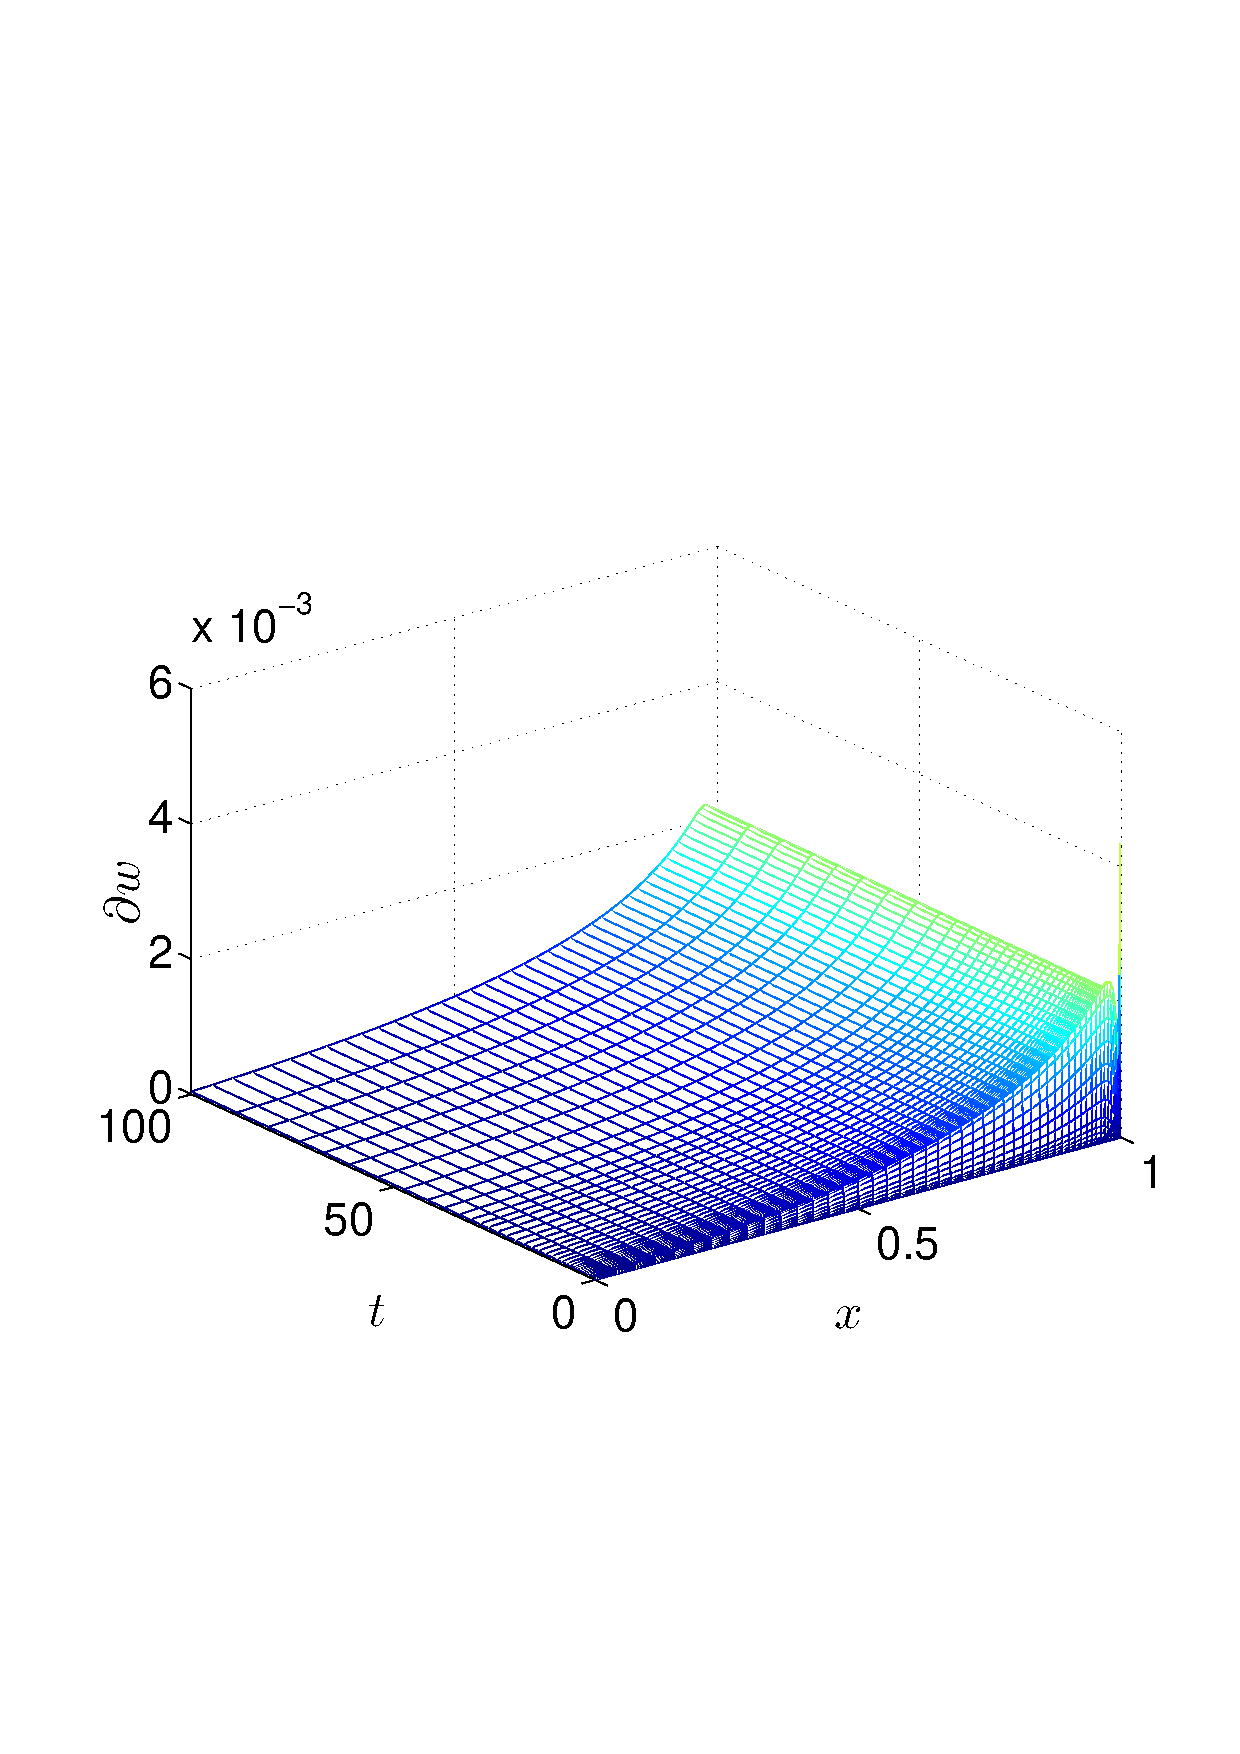
\includegraphics[width=\textwidth]{3_PKN_numerical/extra_carter/q_l_analitical.png}
                \caption{$\delta w_{max}$ for full analytical leak off}
                \label{}
        \end{subfigure}
        \begin{subfigure}[b]{0.33\textwidth}
                \centering
                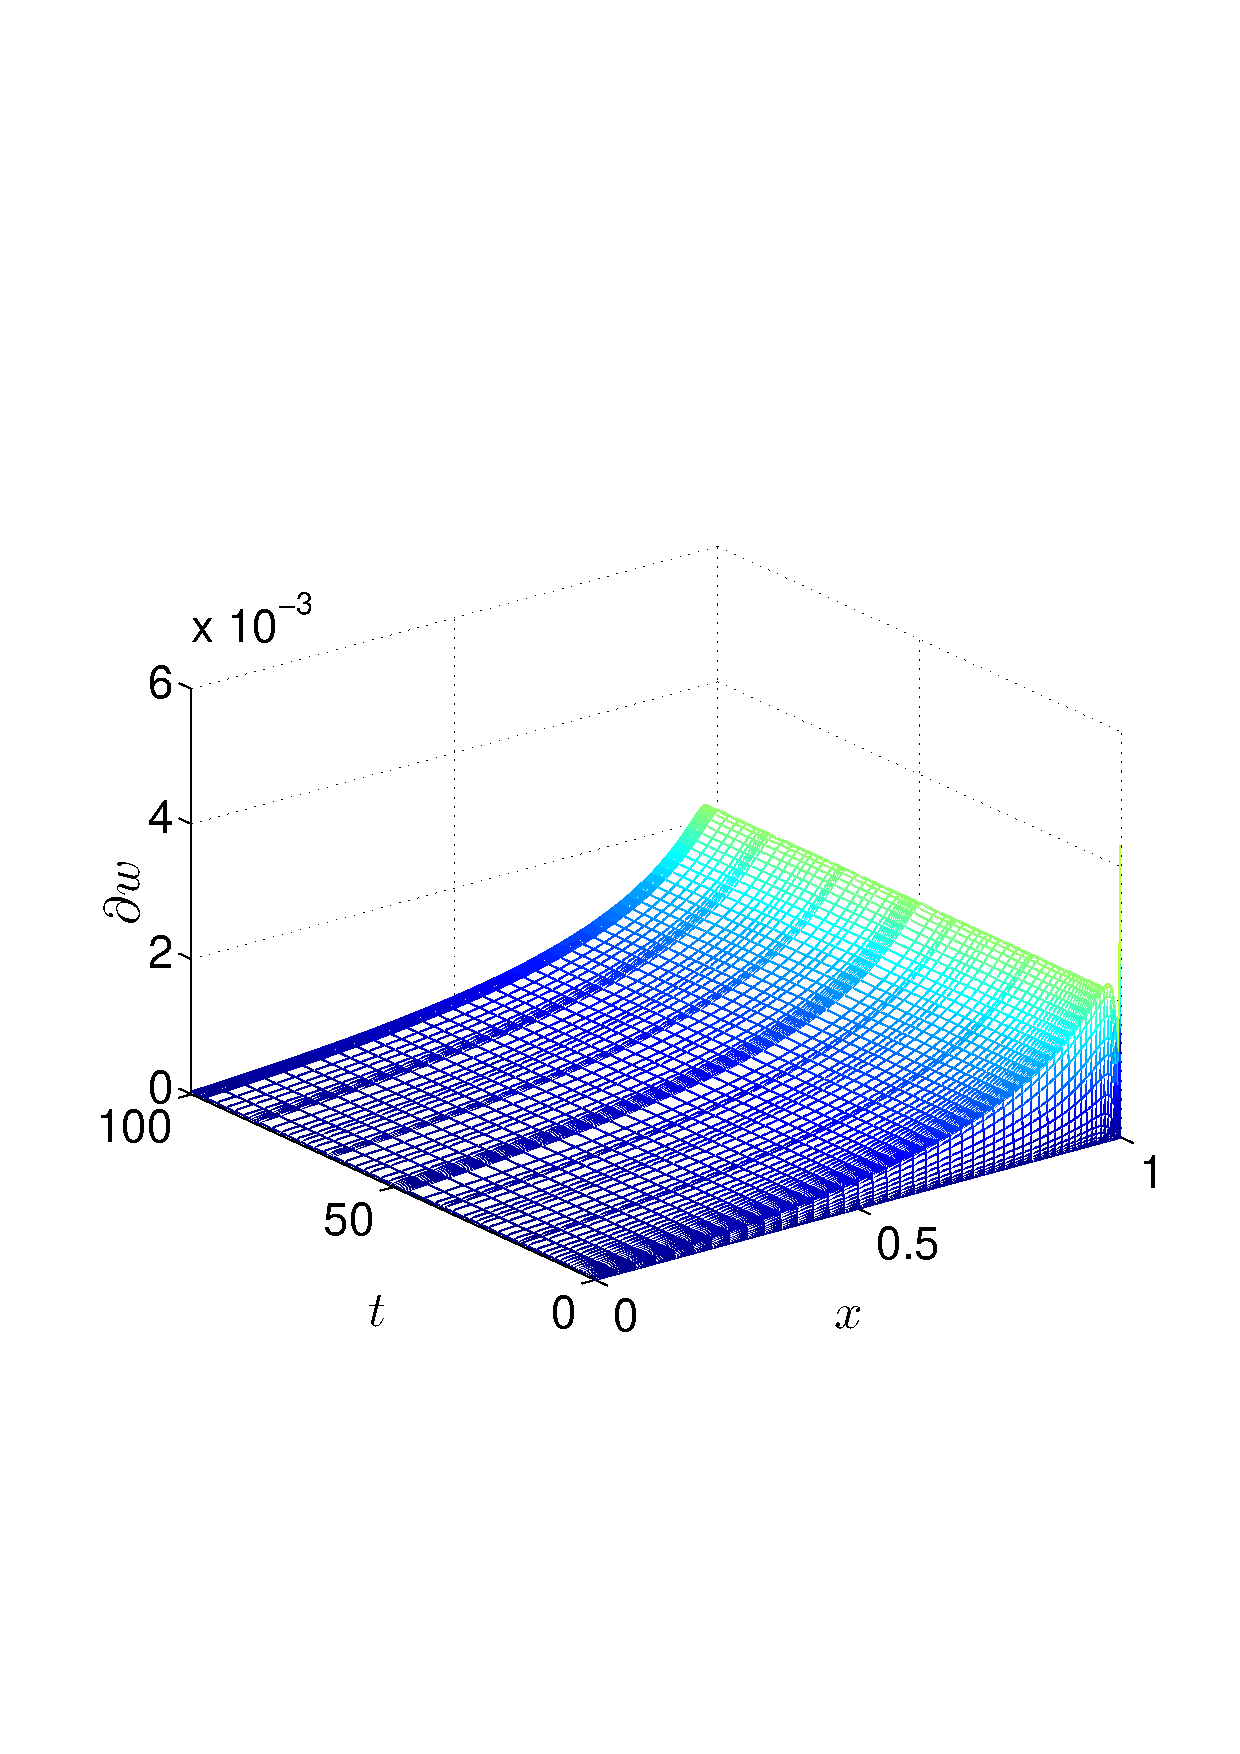
\includegraphics[width=\textwidth]{3_PKN_numerical/extra_carter/q_l_numerical.png}
                \caption{$\delta w_{max}$ for partial numerical leak off}
                \label{}
        \end{subfigure}
        \begin{subfigure}[b]{0.33\textwidth}
                \centering
                \includegraphics[width=\textwidth]{3_PKN_numerical/extra_carter/q_l_timesteps.png}
                \caption{Solver time step result}
                \label{step differences}
        \end{subfigure}
\caption{Results of using a leak off handle (??) on $w$ variable system, accuracy remains unchanged, but the computation time, and number of time steps required is affected}
\label{q_star_test}
\end{figure*}


\subsubsection{Remarks on the sensitivity of the Carter leak-off model.}

It is well known that applicability of the empirical Carter law (\ref{carter})$_1$ in the vicinity of the fracture tip is questionable (see for example,
\citet{Economides2000}, \citet{Kovalyshen_1} and \citet{MKP}). Moreover, when combining Carter's leak-off with some non-local variants of elasticity models (for example, KGD model of hydrofracturing), one obtains an infinite
particle velocity at the crack tip. As a result, the speed equation (\ref{velocity_2}) cannot be applied in such a case.
One of the ways to eliminate the negative consequences of this fact is to assume that the Carter law becomes valid at some distance away from the fracture tip (see for example \citet{MKP}).

The PKN model, which does not exhibit such a drawback, gives however a unique opportunity to assess how the solution is affected by a modification of the classic Carter law in the neighborhood of the fracture tip.

To this end, let us consider two ways of modification of the law. The first one assumes that leak-off function equals zero over some distance from the crack front ($d>\varepsilon$). The second one accepts a constant value of $q_l$ in the same interval. This value is taken in such a manner to preserve the continuity of the leak-off function. Note, that both of these modifications change the volume of fluid loss to the rock formation, with respect to the original state.

The relative deviations of the crack lengths for these modifications from the original one are shown in Fig.~\ref{dev_carter}. Results for two values of $d$: $d=\varepsilon$, $d=10\varepsilon$ (for $\varepsilon=10^{-5}$) are depicted. The symbol $q_{ld}$ in the legend refers to the cases when the leak-off function is complimented by the constant value over $1-d\leq x \leq 1$.


\begin{figure}[h!]
\center
    %\hspace{-2mm}
    \includegraphics [scale=0.35]{3_PKN_numerical/extra_carter/leak_off_okrojony.eps}
    \put(-100,-2){$t$}


    \caption{Relative deviations of the crack lengths for different variants of truncated Carter law.}
\label{dev_carter}
\end{figure}

One can see from this picture that the maximal relative discrepancies (of the level of 1\%) appear at the initial and large time ranges. To explain this phenomenon we can easily compute the additional volume of fluid retained in the fracture as a result of the Carter law amendments. Taking into account (\ref{f_D}), these values are $\Delta Q_l(t)=2D(t)\sqrt{d}$ and $\Delta Q_l(t)=D(t)\sqrt{d}$, for the respective modifications (see (\ref{function_D}) for $D(t)$). Note that $D(t)=\sqrt{u(t)/t}$, which explains the level of deviation for the small time. For large time, the effect of accumulation of the difference of the fluid loss, $\int_0^t\Delta Q_l(\tau)d\tau$ = $O(\sqrt{td})$, plays a crucial role.

The above test proves that the application of the Carter law modified in the aforementioned ways, is fully justified when one considers the accuracies required in the practical applications.
